\documentclass{article}
\usepackage[T1]{fontenc}			% Selecao de codigos de fonte.
\usepackage[utf8]{inputenc}		% Codificacao do documento (conversão automática dos acentos)
\usepackage{longtable}
\usepackage{amsmath,amssymb,mathrsfs, amsthm}	% Comandos matemáticos avançados 
\usepackage{booktabs}
\usepackage{graphicx}	         % Inclusão de gráficos
\usepackage{float}
\usepackage[brazil]{babel}

\begin{document}
	% latex table generated in R 3.4.2 by xtable 1.8-2 package
% Thu Dec 21 22:04:25 2017
\begin{table}[H]
\centering
\caption{Estatísticas descritivas dos retornos (amostra completa de 01/01/2003 a 30/08/2017).} 
\label{tab:descritivas}
\begin{tabular}{lrrrrrr}
  \hline
Descritivas & IBovespa & S\&P500 & S\&P TSE & IPSA & Merval & IPC \\ 
  \hline
Média & 0.00050 & 0.00028 & 0.00022 & 0.00045 & 0.00106 & 0.00058 \\ 
  Mediana & 0.00095 & 0.00066 & 0.00074 & 0.00063 & 0.00149 & 0.00093 \\ 
  Máximo & 0.13677 & 0.10957 & 0.09370 & 0.11803 & 0.10432 & 0.10441 \\ 
  Mínimo & -0.12096 & -0.09470 & -0.09788 & -0.07236 & -0.12952 & -0.07266 \\ 
  Desvp & 0.01739 & 0.01168 & 0.01064 & 0.00976 & 0.01981 & 0.01203 \\ 
  Assimetria & -0.08670 & -0.33132 & -0.71699 & -0.01775 & -0.48666 & 0.03784 \\ 
  Curtose & 4.90756 & 11.61430 & 11.84413 & 10.63489 & 3.63347 & 6.58809 \\ 
  Jarque-Bera & 3655.76824 & 20846.77985 & 21949.89333 & 17262.83228 & 2125.37846 & 6666.52444 \\ 
   & 0.00000 & 0.00000 & 0.00000 & 0.00000 & 0.00000 & 0.00000 \\ 
  Q(10) & 16.27860 & 59.66372 & 30.28797 & 111.10837 & 13.32940 & 42.80163 \\ 
   & 0.00278 & 0.00000 & 0.00000 & 0.00000 & 0.01350 & 0.00000 \\ 
  $Q^2(10)$ & 1299.67247 & 1907.90243 & 2384.89328 & 919.76012 & 752.94283 & 1012.31695 \\ 
   & 0.00000 & 0.00000 & 0.00000 & 0.00000 & 0.00000 & 0.00000 \\ 
  N.obs & 3632.00000 & 3692.00000 & 3696.00000 & 3658.00000 & 3598.00000 & 3680.00000 \\ 
   \hline
\end{tabular}
\end{table}

	
	% latex table generated in R 3.4.3 by xtable 1.8-2 package
% Mon Dec 11 22:38:04 2017
\begin{table}[H]
\centering
\caption{Par\^ametros estimados do modelo eGARCH. Valores p apresentados 
               de acordo com erros padrão robustos. (amostra de trabalho entre 31/08/2003 a 31/08/2013).} 
\label{tab:garchcoef}
\begin{tabular}{lrrrrrr}
  \hline
Parâmetros & IBovespa & S\&P500 & S\&P TSE & IPSA & Merval & IPC \\ 
  \hline
$\mu$ & -0.02941 & -0.02408 & -0.02803 & -0.04435 & -0.08437 & -0.04635 \\ 
   & 0.33805 & 0.08301 & 0.06285 & 0.07210 & 0.04481 & 0.01553 \\ 
  $\phi_1$ & 0.00341 & -0.06726 & 0.00745 & 0.18051 & 0.02976 & 0.05380 \\ 
   & 0.84146 & 0.00017 & 0.70981 & 0.00000 & 0.16595 & 0.00078 \\ 
  $\omega$ & 0.02119 & -0.00233 & -0.00322 & -0.01159 & 0.04476 & 0.00660 \\ 
   & 0.00000 & 0.54715 & 0.29693 & 0.05213 & 0.50349 & 0.02781 \\ 
  $\alpha_1$ & 0.22198 & 0.28021 & 0.19909 & 0.18509 & 0.15027 & 0.16203 \\ 
   & 0.00000 & 0.00000 & 0.00000 & 0.00000 & 0.00002 & 0.00000 \\ 
  $\alpha_2$ & -0.13750 & -0.13789 & -0.11185 & -0.08908 & -0.10071 & -0.06358 \\ 
   & 0.00001 & 0.00030 & 0.00042 & 0.00283 & 0.04321 & 0.02877 \\ 
  $\beta_1$ & 0.97812 & 0.98106 & 0.98309 & 0.95718 & 0.95878 & 0.97938 \\ 
   & 0.00000 & 0.00000 & 0.00000 & 0.00000 & 0.00000 & 0.00000 \\ 
  $\gamma_1$ & -0.05129 & -0.19778 & -0.04319 & 0.19183 & 0.05298 & 0.03944 \\ 
   & 0.29514 & 0.00007 & 0.38635 & 0.00013 & 0.38739 & 0.11206 \\ 
  $\gamma_2$ & 0.19217 & 0.32411 & 0.17950 & 0.04302 & 0.13407 & 0.12604 \\ 
   & 0.00008 & 0.00000 & 0.00026 & 0.36398 & 0.20329 & 0.00003 \\ 
  $\zeta$ & 1.10357 & 1.18792 & 1.24013 & 1.05445 & 1.09390 & 1.16005 \\ 
   & 0.00000 & 0.00000 & 0.00000 & 0.00000 & 0.00000 & 0.00000 \\ 
  $\nu$ & 12.94213 & 7.62352 & 11.77302 & 11.79185 & 5.99271 & 9.13938 \\ 
   & 0.00001 & 0.00000 & 0.00000 & 0.00000 & 0.00000 & 0.00000 \\ 
   \hline
\end{tabular}
\end{table}

	
	% latex table generated in R 3.4.1 by xtable 1.8-2 package
% Thu Dec 21 19:18:43 2017
\begin{table}[H]
\centering
\caption{Estat�sticas de diagn�stico para o modelo eGARCH. 
               (amostra de trabalho entre 01/01/2003 a 31/12/2008 ).} 
\label{tab:garchstats}
\begin{tabular}{lrrrrrr}
  \hline
Estat�stica & IBovespa & S\&P500 & S\&P TSE & IPSA & Merval & IPC \\ 
  \hline
Jarque-Bera & 49.43583 & 215.01376 & 140.05041 & 34.73241 & 745.12915 & 110.65501 \\ 
   & 0.00000 & 0.00000 & 0.00000 & 0.00000 & 0.00000 & 0.00000 \\ 
  Q(10) & 5.06861 & 6.62418 & 2.48467 & 4.76916 & 10.79623 & 6.51737 \\ 
   & 0.49583 & 0.29224 & 0.88747 & 0.54185 & 0.04803 & 0.30402 \\ 
  $Q^2(10)$ & 2.06336 & 4.68145 & 4.45030 & 7.97618 & 3.96265 & 2.65360 \\ 
   & 0.93211 & 0.55561 & 0.59236 & 0.17130 & 0.67109 & 0.86672 \\ 
   \hline
\end{tabular}
\end{table}


	% latex table generated in R 3.4.2 by xtable 1.8-2 package
% Mon Jan  1 13:31:10 2018
\begin{table}[H]
\centering
\caption{Parâmetros estimados para o modelo EVT dos resíduos padronizados. 
               (amostra de trabalho entre 01/01/2003 a 31/12/2008 ).} 
\label{tab:evtcoef}
\begin{tabular}{lrrrrrr}
  \hline
 & IBovespa & S\&P500 & S\&P TSE & IPSA & Merval & IPC \\ 
  \hline
Obs. dentro amostra & 1487.00000 & 1511.00000 & 1522.00000 & 1498.00000 & 1495.00000 & 1514.00000 \\ 
  Limiar & 1.43392 & 1.36357 & 1.48743 & 1.40436 & 1.35673 & 1.40554 \\ 
  Número de excessos & 119.00000 & 121.00000 & 122.00000 & 120.00000 & 120.00000 & 122.00000 \\ 
  Parâmetro forma GPD & -0.01136 & -0.02867 & -0.00749 & 0.00343 & 0.07085 & 0.00287 \\ 
  Erro padrão & 0.07900 & 0.06368 & 0.08595 & 0.08475 & 0.08132 & 0.08418 \\ 
  Parâmetro escala GPD & 0.55190 & 0.72245 & 0.61939 & 0.55517 & 0.65097 & 0.61094 \\ 
  Erro padrão & 0.06679 & 0.08017 & 0.07732 & 0.06915 & 0.07947 & 0.07552 \\ 
  Quantil 97.5\% & 2.07183 & 2.19073 & 2.20595 & 2.05214 & 2.14835 & 2.12178 \\ 
  Quantil 99.0\% & 2.56831 & 2.82263 & 2.76663 & 2.56368 & 2.81771 & 2.68420 \\ 
   \hline
\end{tabular}
\end{table}


	% latex table generated in R 3.4.1 by xtable 1.8-2 package
% Thu Dec 21 19:19:27 2017
\begin{table}[H]
\centering
\caption{Percentual de viola��es. (fora da amostra, dados entre 02/01/2009 e 31/08/2017} 
\label{tab:varviol}
\begin{tabular}{lrrrrrr}
  \hline
Modelo & IBovespa & IPC & IPSA & Merval & S\&P TSE & S\&P500 \\ 
  \hline
Cobertura = 1\% &  &  &  &  &  &  \\ 
  EVT Condicional & 0.47 & 0.23 & 0.37 & 0.48 & 0.41 & 0.37 \\ 
  Normal Condicional & 0.56 & 0.46 & 0.42 & 1.00 & 0.78 & 0.73 \\ 
  t-Student Condicional & 0.56 & 0.46 & 0.42 & 1.00 & 0.78 & 0.73 \\ 
  RiskMetrics & 0.42 & 0.60 & 0.65 & 0.90 & 1.06 & 0.78 \\ 
  EVT Incond. Filtrada & 0.19 & 0.05 & 0.05 & 0.57 & 0.14 & 0.14 \\ 
  Normal Incondicional & 0.19 & 0.09 & 0.05 & 0.76 & 0.05 & 0.14 \\ 
  t-Student Incondicional & 0.09 & 0.05 & 0.00 & 0.52 & 0.00 & 0.00 \\ 
  Cobertura = 2.5\% &  &  &  &  &  &  \\ 
  EVT Condicional & 0.84 & 0.60 & 0.79 & 1.14 & 0.87 & 0.73 \\ 
  Normal Condicional & 0.98 & 0.92 & 0.88 & 1.33 & 1.47 & 0.92 \\ 
  t-Student Condicional & 0.93 & 0.92 & 0.83 & 1.28 & 1.47 & 0.92 \\ 
  RiskMetrics & 0.98 & 1.29 & 0.93 & 1.28 & 1.66 & 1.24 \\ 
  EVT Incond. Filtrada & 0.56 & 0.14 & 0.09 & 0.95 & 0.41 & 0.32 \\ 
  Normal Incondicional & 0.42 & 0.14 & 0.05 & 1.09 & 0.23 & 0.18 \\ 
  t-Student Incondicional & 0.42 & 0.14 & 0.05 & 1.00 & 0.28 & 0.18 \\ 
   \hline
\end{tabular}
\end{table}

	
	% latex table generated in R 3.4.3 by xtable 1.8-2 package
% Fri Jan 12 13:52:36 2018
\begin{longtable}{llrrrrrr}
\caption{Testes estatísticos para o VaR. Teste incondicional de Kupiec, \emph{LRuc}, e teste de
             independência por duração de Christoffersen e Pelletier, \emph{LRdur}. Os modelos testados
são: EVT condicional (cevt), Normal condicional (cnorm), t-Student condicional (ct), Riskmetrics 
(riskmetrics), EVT incondicioanl (uevt), Normal incondicional (unorm) e t-Student incondicional (ut). 
(Período fora da amostra entre 02/01/2009 e 30/08/2017).} \\ 
  \hline
Modelo & Estatística & IBovespa & IPC & IPSA & Merval & S\&P TSE & S\&P500 \\ 
  \hline
Cobertura 1\% &  &  &  &  &  &  &  \\ 
  cevt & LRuc & 0.92 & 0.02 & 1.27 & 1.58 & 0.07 & 0.07 \\ 
  cevt & LRuc p-valor & 0.34 & 0.89 & 0.26 & 0.21 & 0.79 & 0.80 \\ 
  cevt & LRdur & 0.98 & 2.04 & 0.29 & 2.34 & 0.37 & 3.92 \\ 
  cevt & LRdur p-valor & 0.32 & 0.15 & 0.59 & 0.13 & 0.54 & 0.05 \\ 
  cnorm & LRuc & 3.78 & 15.16 & 9.15 & 24.00 & 11.22 & 20.57 \\ 
  cnorm & LRuc p-valor & 0.05 & 0.00 & 0.00 & 0.00 & 0.00 & 0.00 \\ 
  cnorm & LRdur & 2.46 & 0.58 & 0.02 & 1.99 & 0.02 & 0.39 \\ 
  cnorm & LRdur p-valor & 0.12 & 0.44 & 0.90 & 0.16 & 0.89 & 0.53 \\ 
  ct & LRuc & 3.78 & 17.94 & 9.15 & 25.66 & 12.43 & 25.32 \\ 
  ct & LRuc p-valor & 0.05 & 0.00 & 0.00 & 0.00 & 0.00 & 0.00 \\ 
  ct & LRdur & 2.46 & 0.66 & 0.02 & 2.94 & 0.00 & 0.19 \\ 
  ct & LRdur p-valor & 0.12 & 0.42 & 0.90 & 0.09 & 0.96 & 0.66 \\ 
  riskmetrics & LRuc & 4.56 & 20.91 & 19.54 & 29.10 & 34.26 & 32.22 \\ 
  riskmetrics & LRuc p-valor & 0.03 & 0.00 & 0.00 & 0.00 & 0.00 & 0.00 \\ 
  riskmetrics & LRdur & 1.05 & 0.07 & 4.93 & 3.16 & 0.00 & 2.11 \\ 
  riskmetrics & LRdur p-valor & 0.31 & 0.79 & 0.03 & 0.08 & 0.98 & 0.15 \\ 
  uevt & LRuc & 1.53 & 4.07 & 1.61 & 0.72 & 0.80 & 2.18 \\ 
  uevt & LRuc p-valor & 0.22 & 0.04 & 0.21 & 0.40 & 0.37 & 0.14 \\ 
  uevt & LRdur & 1.20 & 3.21 & 10.38 & 8.29 & 35.76 & 28.49 \\ 
  uevt & LRdur p-valor & 0.27 & 0.07 & 0.00 & 0.00 & 0.00 & 0.00 \\ 
  unorm & LRuc & 0.59 & 0.66 & 7.85 & 6.82 & 1.67 & 0.77 \\ 
  unorm & LRuc p-valor & 0.44 & 0.42 & 0.01 & 0.01 & 0.20 & 0.38 \\ 
  unorm & LRdur & 2.49 & 9.73 & 7.92 & 4.70 & 40.84 & 31.79 \\ 
  unorm & LRdur p-valor & 0.11 & 0.00 & 0.00 & 0.03 & 0.00 & 0.00 \\ 
  ut & LRuc & 9.33 & 9.57 & 13.51 & 0.41 & 6.54 & 5.32 \\ 
  ut & LRuc p-valor & 0.00 & 0.00 & 0.00 & 0.52 & 0.01 & 0.02 \\ 
  ut & LRdur & 0.52 & 0.66 & 16.16 & 8.62 & 11.24 & 18.50 \\ 
  ut & LRdur p-valor & 0.47 & 0.41 & 0.00 & 0.00 & 0.00 & 0.00 \\ 
  Cobertura 2.5\% &  &  &  &  &  &  &  \\ 
  cevt & LRuc & 0.01 & 0.00 & 0.02 & 1.33 & 0.36 & 0.24 \\ 
  cevt & LRuc p-valor & 0.93 & 0.99 & 0.89 & 0.25 & 0.55 & 0.63 \\ 
  cevt & LRdur & 0.39 & 0.55 & 0.03 & 2.82 & 0.36 & 0.27 \\ 
  cevt & LRdur p-valor & 0.53 & 0.46 & 0.86 & 0.09 & 0.55 & 0.60 \\ 
  cnorm & LRuc & 0.11 & 4.38 & 0.67 & 8.71 & 10.10 & 13.21 \\ 
  cnorm & LRuc p-valor & 0.74 & 0.04 & 0.41 & 0.00 & 0.00 & 0.00 \\ 
  cnorm & LRdur & 0.43 & 0.14 & 0.37 & 0.54 & 0.86 & 0.01 \\ 
  cnorm & LRdur p-valor & 0.51 & 0.71 & 0.55 & 0.46 & 0.35 & 0.92 \\ 
  ct & LRuc & 0.11 & 3.86 & 0.17 & 7.99 & 10.10 & 13.21 \\ 
  ct & LRuc p-valor & 0.74 & 0.05 & 0.68 & 0.00 & 0.00 & 0.00 \\ 
  ct & LRdur & 0.43 & 0.10 & 0.32 & 0.51 & 0.86 & 0.01 \\ 
  ct & LRdur p-valor & 0.51 & 0.75 & 0.57 & 0.48 & 0.35 & 0.92 \\ 
  riskmetrics & LRuc & 4.17 & 8.79 & 5.60 & 6.63 & 21.18 & 23.10 \\ 
  riskmetrics & LRuc p-valor & 0.04 & 0.00 & 0.02 & 0.01 & 0.00 & 0.00 \\ 
  riskmetrics & LRdur & 7.73 & 1.55 & 3.58 & 1.00 & 0.26 & 2.50 \\ 
  riskmetrics & LRdur p-valor & 0.01 & 0.21 & 0.06 & 0.32 & 0.61 & 0.11 \\ 
  uevt & LRuc & 5.90 & 13.12 & 2.95 & 0.00 & 0.05 & 0.39 \\ 
  uevt & LRuc p-valor & 0.02 & 0.00 & 0.09 & 0.95 & 0.82 & 0.53 \\ 
  uevt & LRdur & 16.55 & 14.30 & 20.53 & 6.93 & 30.09 & 42.63 \\ 
  uevt & LRdur p-valor & 0.00 & 0.00 & 0.00 & 0.01 & 0.00 & 0.00 \\ 
  unorm & LRuc & 6.69 & 6.24 & 19.86 & 3.27 & 0.36 & 3.19 \\ 
  unorm & LRuc p-valor & 0.01 & 0.01 & 0.00 & 0.07 & 0.55 & 0.07 \\ 
  unorm & LRdur & 14.09 & 19.01 & 8.98 & 13.89 & 40.84 & 31.24 \\ 
  unorm & LRdur p-valor & 0.00 & 0.00 & 0.00 & 0.00 & 0.00 & 0.00 \\ 
  ut & LRuc & 9.39 & 7.91 & 15.52 & 2.40 & 0.10 & 5.01 \\ 
  ut & LRuc p-valor & 0.00 & 0.00 & 0.00 & 0.12 & 0.75 & 0.03 \\ 
  ut & LRdur & 13.54 & 19.03 & 6.98 & 17.92 & 42.74 & 31.96 \\ 
  ut & LRdur p-valor & 0.00 & 0.00 & 0.01 & 0.00 & 0.00 & 0.00 \\ 
   \hline
\hline
\label{tab:vartest}
\end{longtable}

	
	\begin{table}[H]

\caption{\label{tab:vartest_suma}Sumário para o número de rejeições das hipóteses nulas de um modelo 
corretamente especificado. Nível de confiança a 95\%. De seis índices com 
dois testes, resulta em um total de doze rejeições possíveis. 
(Período fora da amostra entre 02/01/2009 e 30/08/2017).}
\centering
\begin{tabular}[t]{ccccc}
\toprule
\multicolumn{1}{c}{} & \multicolumn{2}{c}{Cobertura 1\%} & \multicolumn{2}{c}{Cobertura 2.5\%} \\
\cmidrule(l{2pt}r{2pt}){2-3} \cmidrule(l{2pt}r{2pt}){4-5}
Modelo & LRdur & LRuc & LRdur & LRuc\\
\midrule
cevt & 1 & 0 & 0 & 0\\
cnorm & 0 & 5 & 0 & 4\\
ct & 0 & 5 & 0 & 4\\
riskmetrics & 1 & 6 & 1 & 6\\
uevt & 4 & 1 & 6 & 2\\
\addlinespace
unorm & 5 & 2 & 6 & 3\\
ut & 4 & 5 & 6 & 4\\
\bottomrule
\end{tabular}
\end{table}

	

	\begin{figure}[H]
		\centering
		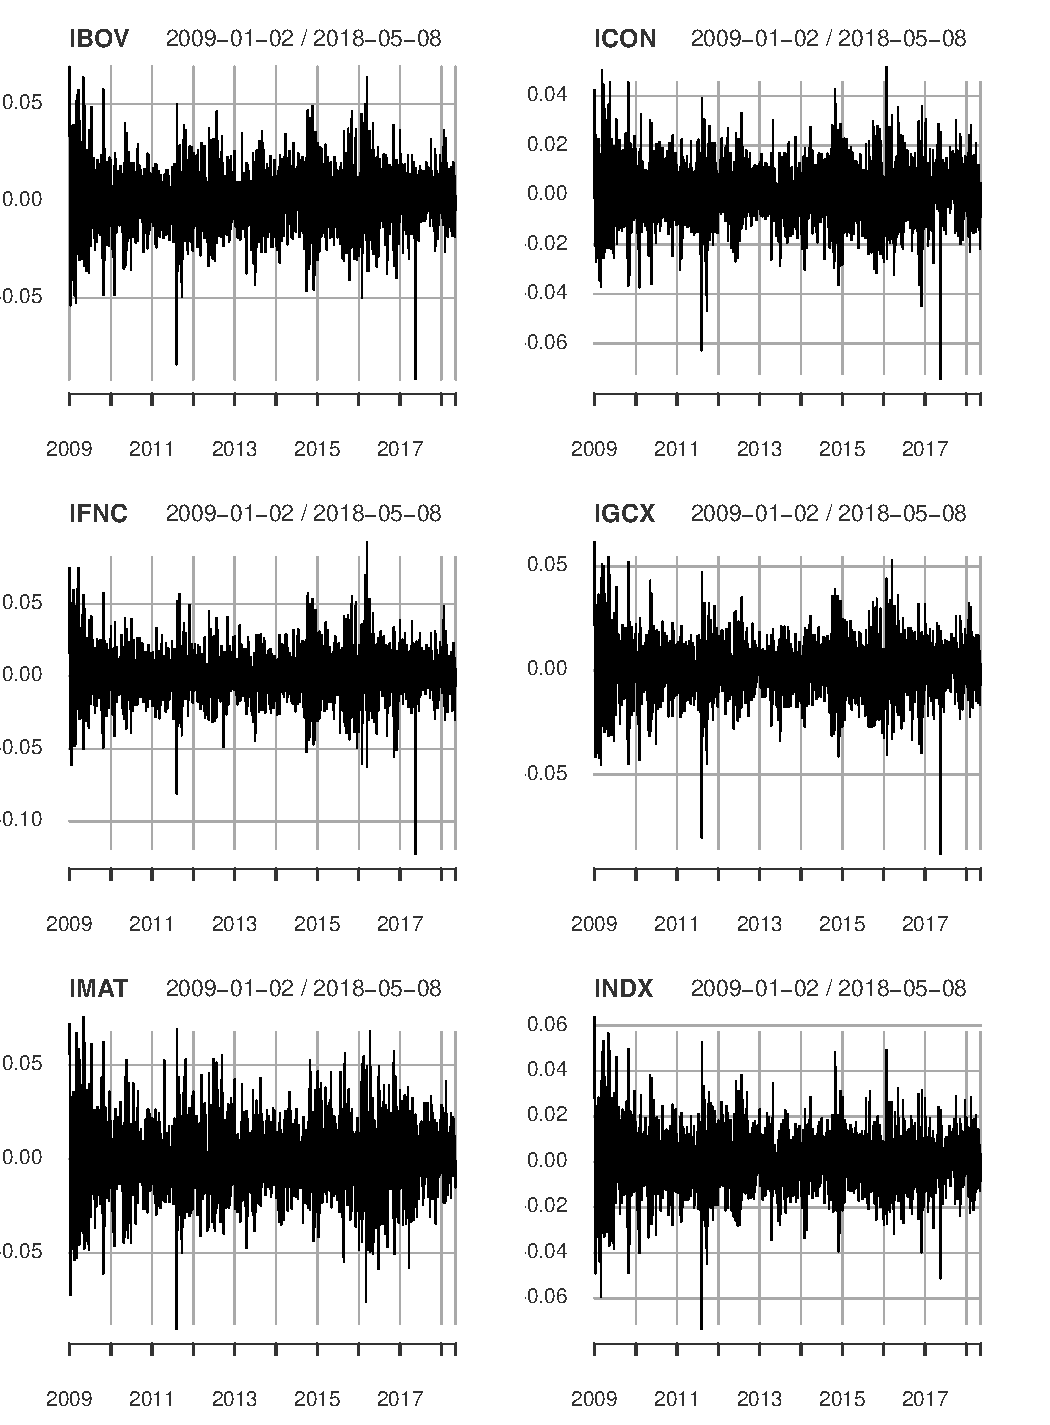
\includegraphics[width=1\linewidth]{figs/artigo-retornos}
		\caption{Retornos dos índices do estudo. Período completo entre 01/01/2003 a 30/08/2017.}
		\label{fig:artigo-retornos}
	\end{figure}

	\begin{figure}[H]
		\centering
		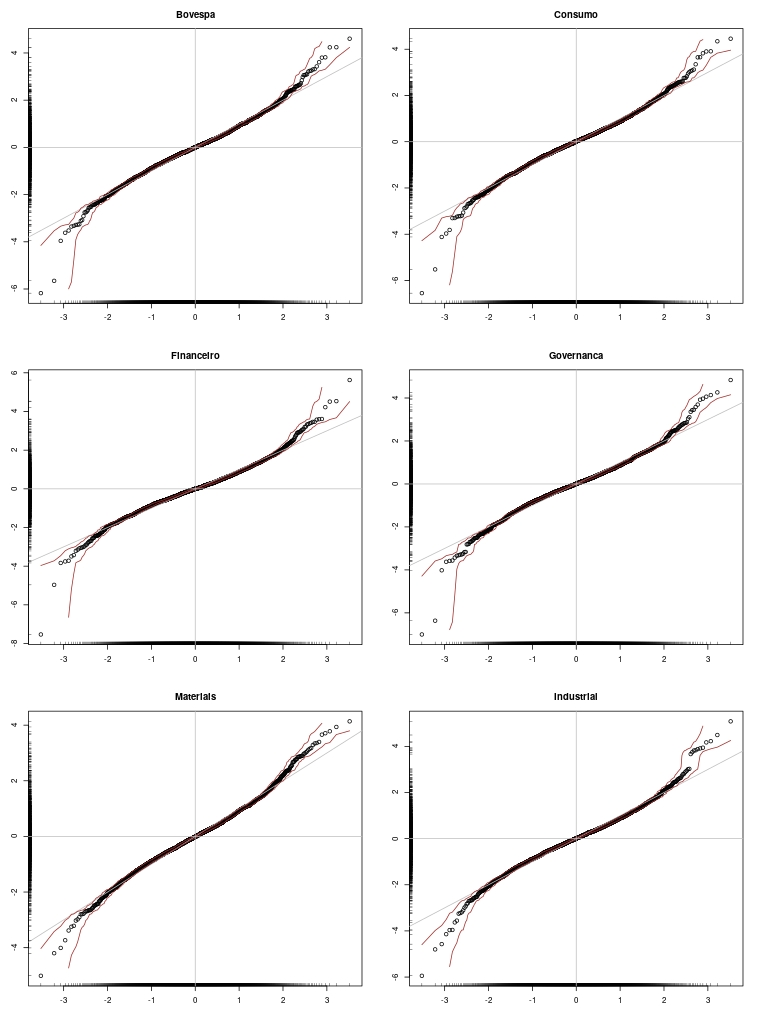
\includegraphics[width=1\linewidth]{figs/artigo-qqplots}
		\caption{Análise de normalidade dos retornos através de gráficos quantil-quantil.}
		\label{fig:artigo-qqplots}
	\end{figure}

	\begin{figure}[H]
		\centering
		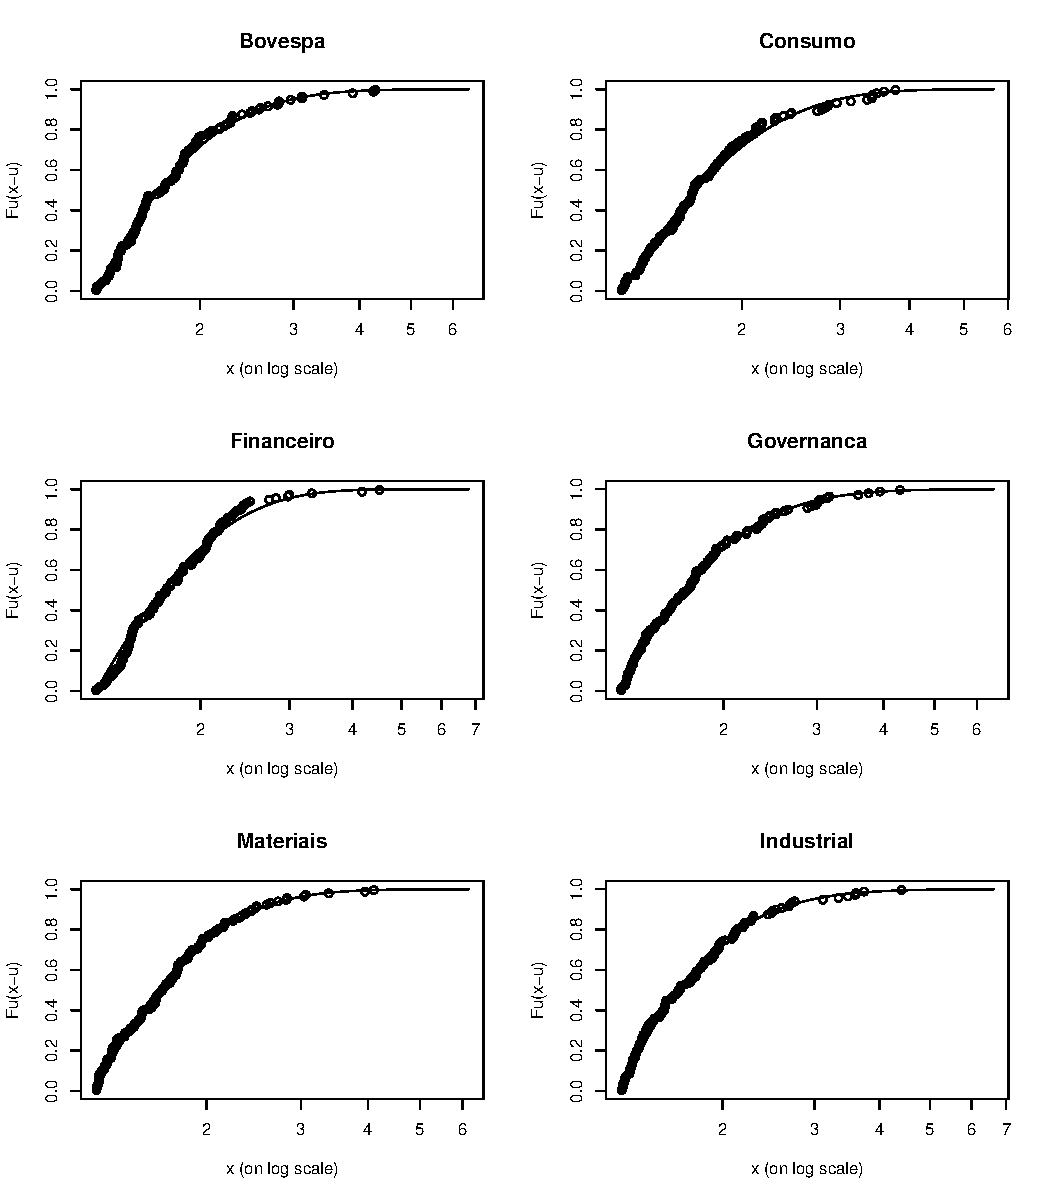
\includegraphics[width=1\linewidth]{figs/artigo-gpdfit}
		\caption{Qualidade do ajuste dos dados de inovações em excesso contra uma GPD de referência. Período dentro da amostra.}
		\label{fig:artigo-gpdfit}
	\end{figure}

	\begin{figure}[H]
		\centering
		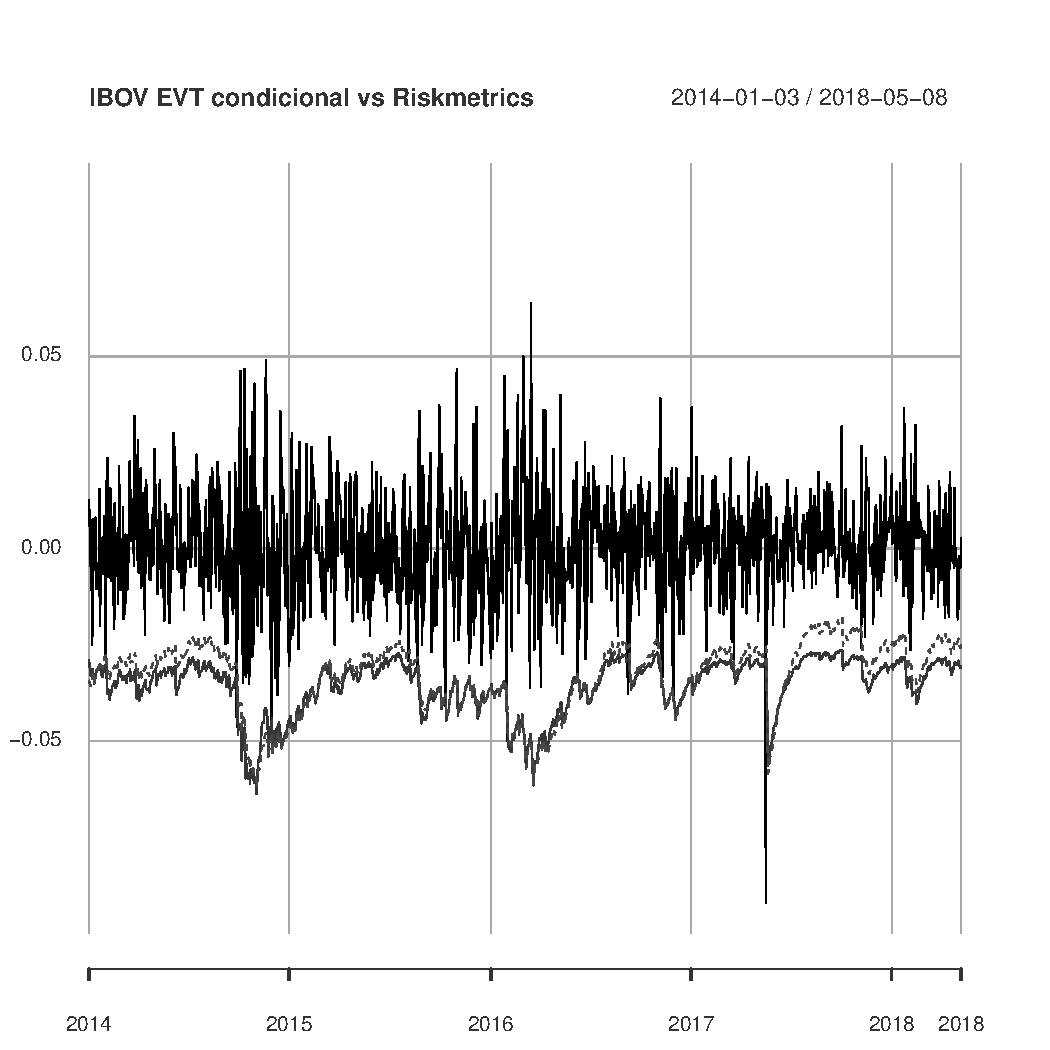
\includegraphics[width=1\linewidth]{figs/artigo-ibovevt}
		\caption{Teste fora da amostra para o Ibovespa. O modelo EVT condicional (linha pontilhada) é muito mais \textbf{reativo a mudanças na volatilidade que o modelo EVT incondicional filtrado (linha tracejada)}.}
		\label{fig:artigo-sp500evt}
	\end{figure}

\end{document}